\documentclass[12pt]{article} 
\usepackage{graphicx}
\usepackage[utf8]{inputenc} 
  
\title{\textbf{Labwork 3}}
\author{Truong Quang Nam\\Student ID: 2540080}
\date{}


\begin{document}
\maketitle
\section{Device}
\begin{itemize}
    \item \textbf{GPU} NVIDIA GeForce GTX 1650
    \item \textbf{CPU} Ryzen 7 4800h
\end{itemize}
Image to process
\begin{figure}[htbp]
    \centering
    \includegraphics[width=0.8\textwidth]{Image.jpg}
    \caption{A image to process}
    \label{fig:mo_ta_anh}
\end{figure}


\section{Cpu compute}
This part to convert the normal image "Image.jpg" to gray image by cpu\\
Step to do:
\begin{verbatim}
img = mpimg.imread('Image.jpg')
height, width, channels = img.shape
pixel_count = img.shape[0] * img.shape[1]
\end{verbatim}
Load image and compute size and number pixel of image
\begin{verbatim}
img_flattened = img.reshape(-1, 3)
gray_flattened = np.zeros(pixel_count,dtype=np.float32)
\end{verbatim}
Flat the image in 1D and create a gray image to save the output

\begin{verbatim}
start_time  = time.time()
for index in range(pixel_count):
    r = img_flattened[index,0] / 3.0
    g = img_flattened[index,1] / 3.0
    b = img_flattened[index,2] / 3.0
    gray_flattened[index] = r + g + b
end_time = time.time()
\end{verbatim}
Start time counter and compute avagerate r g b and put to save to gray image with each index
\begin{verbatim}
gray_img = gray_flattened.reshape(height, width).astype(np.uint8)
plt.figure(figsize=(6, 6))
plt.title("Gray image ")
plt.imshow(gray_img, cmap='gray')
plt.axis('off')
plt.imsave('gray_iamge_cpu.png', gray_img, cmap='gray')
plt.show()
\end{verbatim}
Display and save the image

\section{GPU Compute}
This part to convert the normal image "Image.jpg" to gray image by gpu\\
Step to do:
\begin{verbatim}
@cuda.jit
def gray_image(image_flat, gray_flat, pixel_count):

    index = cuda.grid(1)

    if index < pixel_count:

        r = image_flat[index, 0]
        g = image_flat[index, 1]
        b = image_flat[index, 2]

        gray_flat[index] = (r + g + b) / 3.0

\end{verbatim}
Here is function to compute in gpu.
Read image as cpu
\begin{verbatim}
d_img_flattened = cuda.to_device(img_flattened)
d_gray_flattened = cuda.device_array(pixel_count, dtype=np.float32)

\end{verbatim}
Load image to gpu memory, create memory in gpu to save output in
\begin{verbatim}
threads_per_block = 256
blocks_per_grid = (pixel_count + (threads_per_block - 1)) 

gray_image[blocks_per_grid, threads_per_block](
    d_img_flattened,
    d_gray_flattened,
    pixel_count
)

cuda.synchronize()

gray_flattened_cpu = d_gray_flattened.copy_to_host()

\end{verbatim}
Define thread to process and call function to run, synchronize wait for all done, then copy from gpu memory to host memory
The part to display and save are the same as cpu

\section{Result}
CPU time: 86ms
\begin{figure}[htbp]
    \centering
    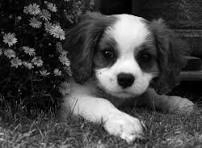
\includegraphics[width=0.8\textwidth]{gray_iamge_cpu.png}
    \caption{CPU process}
    \label{fig:mo_ta_anh}
\end{figure}
GPU Time: 463ms
\begin{figure}[htbp]
    \centering
    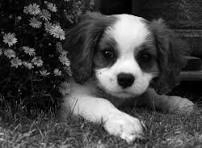
\includegraphics[width=0.8\textwidth]{gray_image_gpu.png}
    \caption{GPU process}
    \label{fig:mo_ta_anh}
\end{figure}
\end{document}